\section{Origin of electromyography}

%HEAD
write head: head
also make sure Martin is not lying about origin of the EMG signal (motor unit action potential VS calcium release from the SR)

The electric potential detected with electromyography is an action potential causing the muscle to contract. Certain mechanisms are involved for this to happen. The motor unit of the muscle needs to be activated alongside with its associated alpha motor system, which is the lower motor neuron, its axon, and the muscle fibers the motor unit innervates. The muscle fiber is an excitable cell with a resting potential of between -90mV and -70mV. A threshold of approximately -55mV needs to be reached for an action potential to be generated. The sarcolemma, the membrane covering the muscle fibers, has sodium and potassium ion channels that maintains the resting potential, depolarize the muscle fiber if the threshold is exceeded or repolarize the muscle fiber. \cite{cram2012}


\begin{figure}[H]
	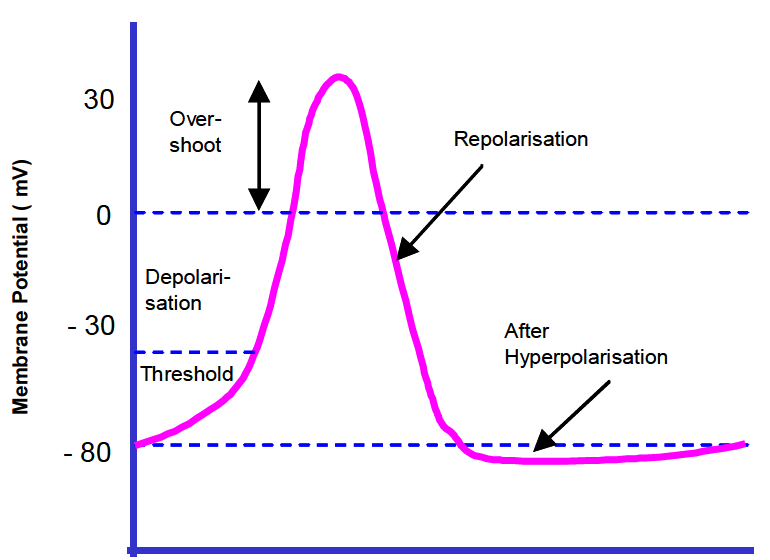
\includegraphics[width=.4\textwidth]{figures/Anatomy/action_potential}  %<--but is not needed.
	\caption{Illustration of the action potential exceeding the threshold for it to be generated and the following depolarization and repolarization. \cite{martini}}
	\label{fig:action_potential}  %<--give the figure a label, so you can reference!
\end{figure}

The lower motor axon is branching out so that it can attach to the muscle fiber at the motor end-plate and create neuromuscular synapses. The action potential traveling down the axon reaches the synapses and releases Acetylcholine (ACh). ACh raises the permeability of the cell membrane where sodium ions influx and causes the membrane to depolarize. Calcium ions are released and binds with troponin and exposes the active sites on the thin filaments which allows the muscle to contract. The action potential travels along the whole muscle fiber through t-tubuluses. This happens in both directions from the motor end-plate to the tendentious attachment. When the peak of the depolarization of about 30mV is reached a rapid efflux of potassium ions causes the muscle fiber to repolarize and reach its resting potential again. \cite{cram2012}

\begin{figure}[H]
	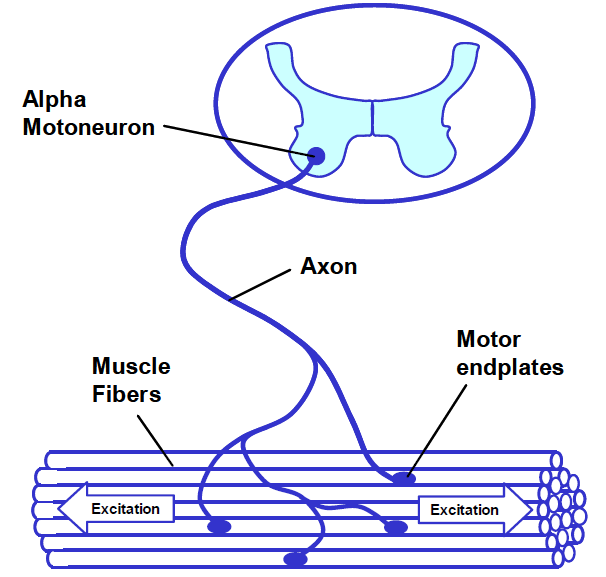
\includegraphics[width=.4\textwidth]{figures/Anatomy/EMG_generation}  %<--but is not needed.
	\caption{Illustration of the action potential exciting the muscle fiber, which causes the release of calcium ions and the muscle to contract. \cite{martini}}
	\label{fig:EMG_generation}  %<--give the figure a label, so you can reference!
\end{figure}

Depending on the force that needs to be applied for a given task more or less motor units are activated and therefore more or less muscle fibers are contracted. The bigger the force the more motor units are activated. Furthermore, the number muscle fibers per motor unit varies between muscles in the human anatomy. The finer the movement the higher the innervation, e.g. the lower arm muscles has a higher innervation than those in the quadriceps. \cite{cram2012}

%the extraocular muscle has the highest innervation of 3:1 and the gastrocnemius muscles has one of 2000:1. \cite{cram2012}

%(Something about how the innervation is in certain muscles of the forearm. Also argue that humans can perform more dexterous movement when the ratio of muscle fibers to motor units is low) (maybe around 100:1)

%(something about how the EMG signal is affected when the limb is positioned differently)
As mentioned this project focuses on the mapping of different hand gestures. This mapping relies on that the generated EMG from the different hand gestures are differentiable. For a prosthetic user a good performing prosthesis must perform hand gestures as well in an elevated limb position as in a seated position to be able to support the user in daily tasks, e. g. taking a cup from a cupboard and pouring water into the cup. However, changes in the EMG occurs when performing the same hand gestures in different limb positions. These signal alternations can occur for different reasons. Changing the limb position can lengthen the muscles and result in a change in the signal source relative to the electrode from which the EMG signal is obtained, and even the lengthening of the muscles itself due to changing limb position will alter the EMG activity caused by a degree of overlap of the thick and thin filaments. Other findings has shown that the activity of certain muscles' is depending on angles of joints besides those primarily actuating the contraction of these muscles. Thus, this limb position effect must be seen as an important aspect to take into consideration in the mapping of hand gestures to control a prosthesis for the user to receive a good performing support device.